\subsection{GUI}
Som udgangspunkt til at lave \glslink{gui}{gui'en} er der blevet implementeret en webside, hvor selve kommunikation mellem databasen, websiden og clienten ser ud som det kan ses i diagrammet på figur \ref{fig:web}.

\begin{figure}[H]
    \centering
    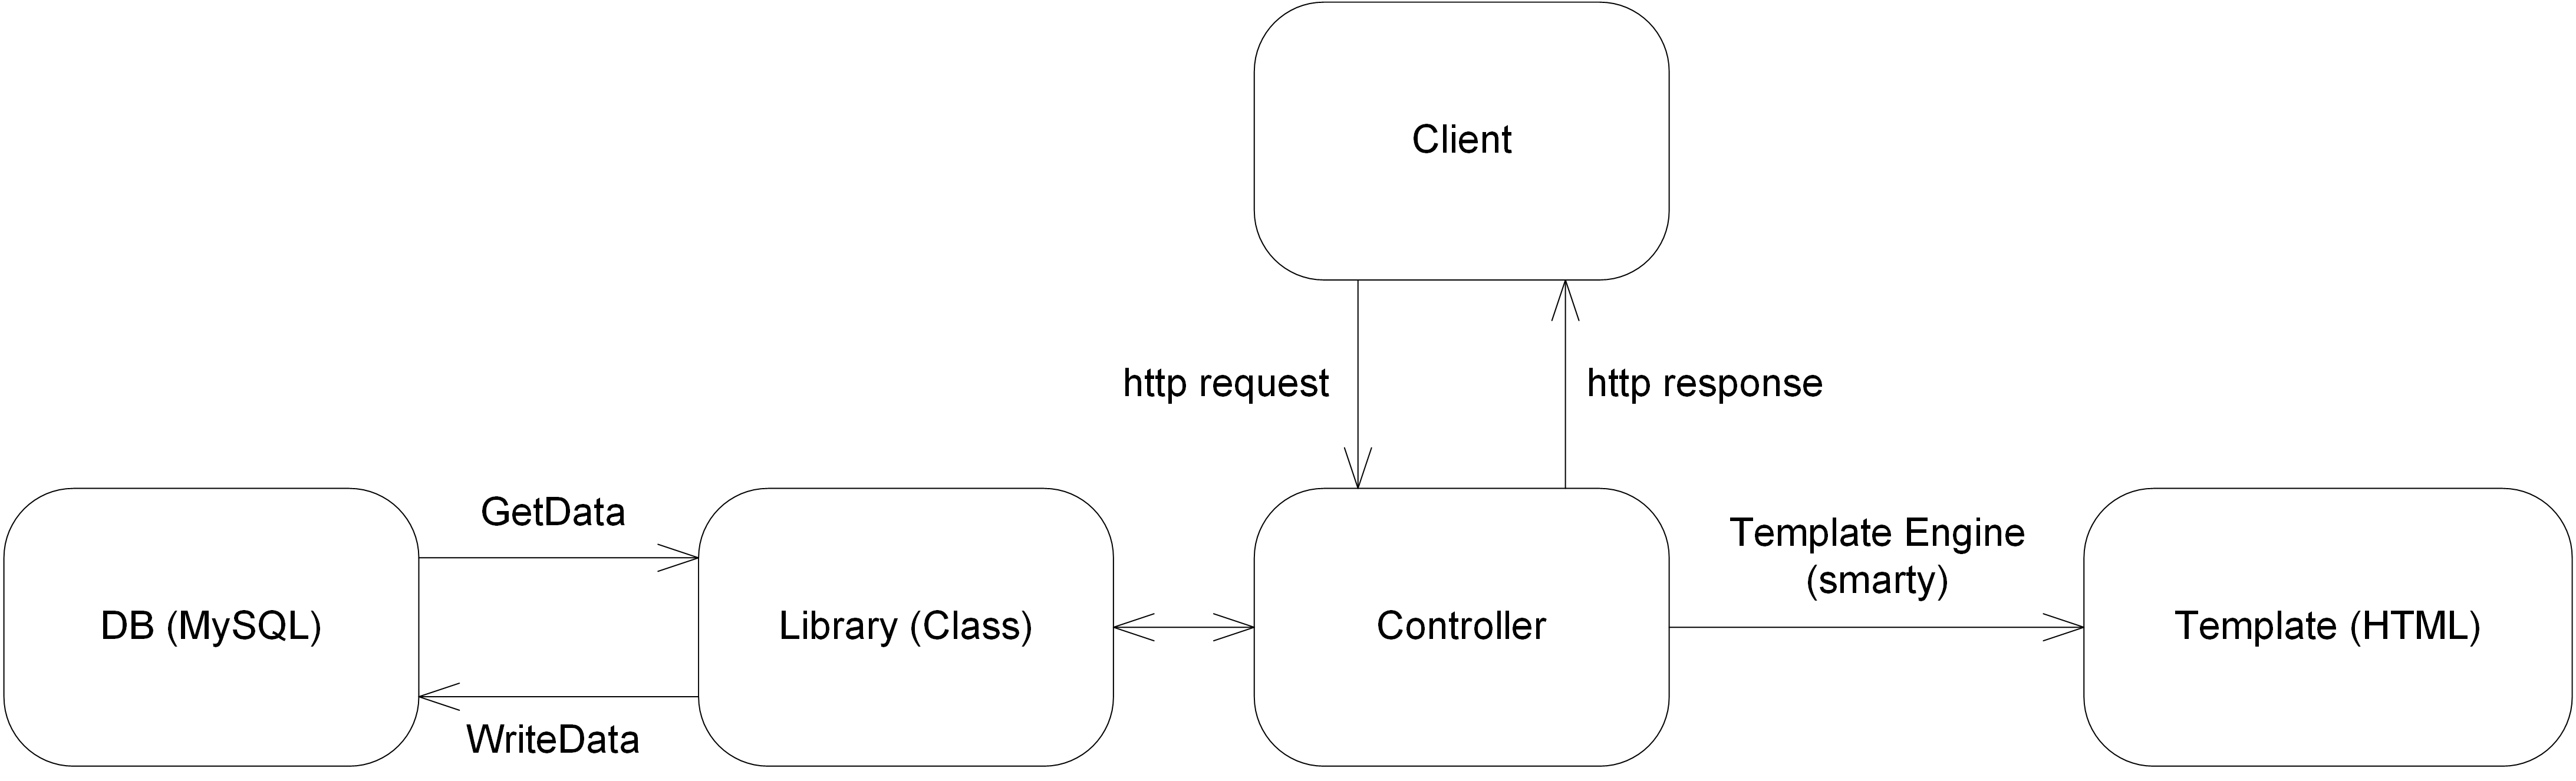
\includegraphics[width=0.8\textwidth]{SoftwareArkitektur/GUI/Intro_GUI_DB/photo/webDiagram.PNG}
    \caption{Diagram over gui og databasens interaktion}
    \label{fig:web}
\end{figure}

I Libary ligger der nogle klasser så det er muligt at oprette objekter, ud fra indholdet i DB\footnote{Databasen}, inde i Controlleren. Controlleren indeholder alle PHP filerne som indeholder funktioner til at sætte websiden op og henter/opdaterer data fra databaserne.
\\\\
Under Template ligger alle HTML filerne som strukturerer indholdet på websiden og visualiserer \glslink{gui}{gui'en}. Hertil er smarty anvendt som Template Engine, det den gør, er at det tager et PHP script, udfører det, og derefter sender forskellige genererede variabler til template (HTML filerne), hvor Smarty derefter udfører forskellige opgaver med variablerne, for til slut at kompilere skabelonen til \glslink{gui}{gui'en}.
\\\\
Til template er der også anvendt Bootstrap\footnote{http://getbootstrap.com/}, som er beregnet til at gøre webudvikling lettere, da den består af HTML- og CSS- baserede design skabeloner til typografi, formularer, knapper, navigation og andre interface komponenter, samt valgfri JavaScript udvidelser.
\\\\
For at sikre at Brugeren ikke skal opdatere websiden, hver gang de vil aflæse nogle nye data eller trykke på en af knapperne er der blevet anvendt nogle jQuery AJAX metoder, som kan bruges til at udveksle data med en server og opdatere dele af en webside uden at genindlæse hele siden.

\subsection{Database}
FlexPMS databasen er blevet anvendt til at opbevare indtastede data omkring kar og sensorøerne med deres ventil og vandingsstatus, samt aflæste værdier fra de forskellige sensorer, hvor denne database kan tilgås via \glslink{gui}{gui'en}. MySQL er databaseformatet der er valgt, og valget bunder i at denne har alle de kvaliteter systembeskrivelsen og kravspecifikationen foreskriver. Desuden er softwaren til etablering af en sådan server gratis, veldokumenteret og nem at gå til.
\\\\
Databasen indeholder nogle forskellig tabeller som er bestemt ud fra de krav vi skulle tilfredsstilles i kravspecifikation og det design der er lavet i systemarkitekturen. Disse tabeller, deres kolonnenavne og deres datatype er illustreret i figur \ref{fig:DB}. 

\begin{figure}[H]
    \centering
    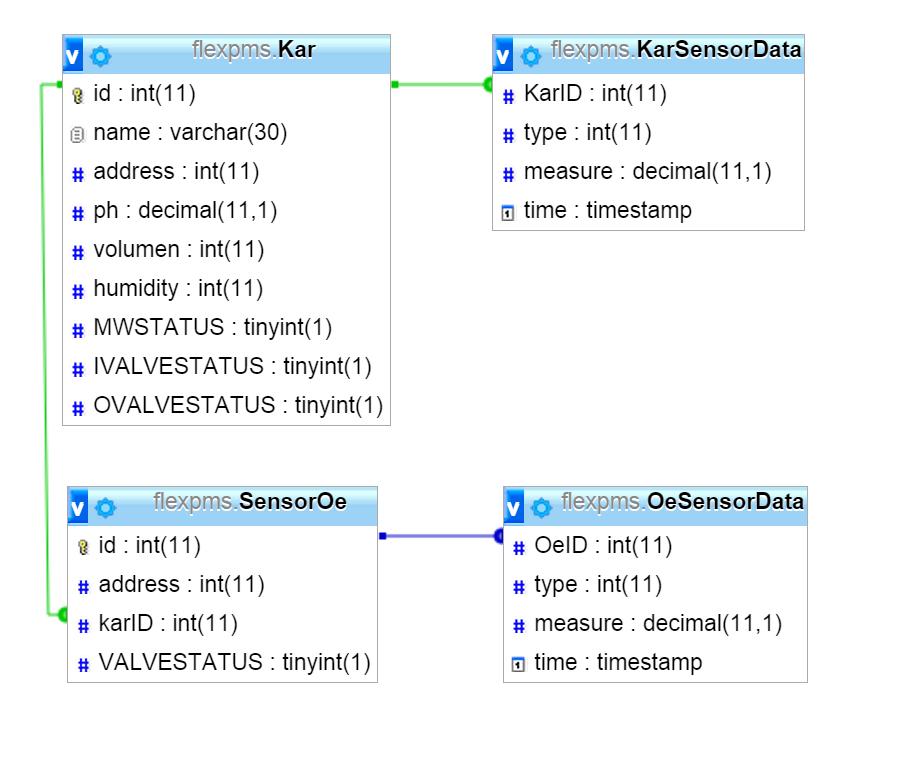
\includegraphics[width=0.7\textwidth]{SoftwareArkitektur/GUI/Intro_GUI_DB/photo/DB_diagram.PNG}
    \caption{Diagram over FlexPMS databasen}
    \label{fig:DB}
\end{figure}

Som det fremgår af diagrammet kender tabellerne til hinanden, det gør de via deres id. Hver \gls{sensoroe} og \gls{kar} har et unikt id for at sikre man kan differentiere mellem dem. Grunden til at dette er vigtigt er fordi at det sikre at data ikke bliver dubleret, ført forkert ind i tabellerne, eller har nogle forkerte interaktioner.
\\\\
En kort beskrivelse af tabellerne og deres kolonner i databasen følger:

\subsubsection{Kar}
Kar indeholder alle kar, deres kar data, som brugeren har oprettet og status for dens ventiler. Alle kar har et navn og adresse med de data som Brugeren ønsker at karet skal have. Kolonnenavnene er beskrevet i tabel \ref{table:kar_kol}.

\begin{table}[H]
\center
\footnotesize
	\begin{tabular}{ | >{\raggedright}p{2.5cm} | >{\raggedright\arraybackslash}p{9.5cm} | }
    \hline
    \vskip 1px \textbf{Kolonnenavn} 	\vskip 0.5px 			& \vskip 0.5px \textbf{Beskrivelse} \vskip 1px 	\\ \hline
    \textit{id} 						& Et unikt id for hver kar tabellen indeholder   						\\ \hline
   	\textit{name} 						& Navnet på karet   													\\ \hline
   	\textit{adresse}	 				& Adressen til karet    												\\ \hline
   	\textit{ph} 						& Den indtastede pH-værdi som Brugeren ønsker    						\\ \hline
   	\textit{volumen} 					& Det vandniveau/antal liter vand som Brugeren ønsker i karet 			\\ \hline
   	\textit{humidity} 					& Den jordfugtighed brugeren ønsker ved \glslink{sensoroe}{Sensor Øerne}\\ \hline
   	\vskip 4pt \textit{MWSTATUS} 		& \vskip 1px
											\begin{minipage}{9cm}
   												Status for manuel vanding:	
    											\begin{itemize}
   													\item 1: Manuel vanding er startet
   													\item 0: Manuel vanding er stoppet
   												\end{itemize}
   												\vskip 1px
 											\end{minipage}   													\\ \hline
 	\vskip 4pt \textit{IVALVESTATUS} 		& \vskip 1px 
											\begin{minipage}{9cm}
   												Status for indløbsventil:	
    											\begin{itemize}
   													\item 1: Indløbsventilen er åben
   													\item 0: Indløbsventilen er lukket
   												\end{itemize}
   												\vskip 1px
 											\end{minipage}   													\\ \hline
 	\vskip 4pt \textit{OVALVESTATUS} 		& \vskip 1px 
											\begin{minipage}{9cm}
   												Status for afløbsventil:	
    											\begin{itemize}
   													\item 1: Afløbsventilen er åben
   													\item 0: Afløbsventilen er lukket
   												\end{itemize}
   												\vskip 1px
 											\end{minipage}   
 																												\\ \hline
\end{tabular}
\caption{Beskrivelser af kolonnenavne for tabellen Kar}
\label{table:kar_kol}
\end{table}


\subsubsection{SensorOe} 
SensorOe indeholder alle Sensor Øer, deres data brugeren har oprette og status for dens ventil. hver Sensor Ø har også et KarID så man kan se hvilket Kar de hører til. Kolonnenavnene er beskrevet i tabel \ref{table:SensorOe_kol}.
\begin{table}[H]
\center
\footnotesize
	\begin{tabular}{ | >{\raggedright}p{2.5cm} | >{\raggedright\arraybackslash}p{9.5cm} | }
    \hline
    \vskip 1px \textbf{Kolonnenavn} \vskip 0.5px & \vskip 0.5px \textbf{Beskrivelse}  \vskip 1px 				\\ \hline
    \textit{id} 						& Et unikt id for hver Sensor Ø tabellen indeholder   					\\ \hline
   	\textit{adresse} 					& Adressen til Sensor Ø    													\\ \hline
   	\textit{KarID}	 					& En reference til det Kars id som Sensor Øen sidder på   				\\ \hline
   	\vskip 4pt \textit{VALVESTATUS} 	& \vskip 1px
											\begin{minipage}{9cm}
   												Status ventilen ved Sensor Øen:	
    											\begin{itemize}
   													\item 1: Ventilen er åben
   													\item 0: Ventilen er lukket
   												\end{itemize}
   												\vskip 1px
 											\end{minipage}   													\\ \hline
\end{tabular}
\caption{Beskrivelser af kolonnenavne for tabellen SensorOe}
\label{table:SensorOe_kol}
\end{table}


\subsubsection{KarSensorData}
KarSensorData indholder alle de målte værdier ved hver kar, derfor har de et KarID, som man kan se hvilken værdi det tilhører. Her indikerer type hvilken slags måling det er, hvor measure værdien der bliver målt. Ydermere er der time der angiver tiden hvor de tilhørende data blev sat ind, på den måde kan man altid tilgå de nyeste data. Kolonnenavnene er beskrevet i tabel \ref{table:karSensorData_kol}.
\begin{table}[H]
\center
\footnotesize
	\begin{tabular}{ | >{\raggedright}p{2.5cm} | >{\raggedright\arraybackslash}p{9.5cm} | }
    \hline
    \vskip 1px \textbf{Kolonnenavn} \vskip 0.5px & \vskip 0.5px \textbf{Beskrivelse}  \vskip 1px 				\\ \hline
    \textit{KarID} 						& En reference til det Kars id der bliver målt på    					\\ \hline
    \vskip 4pt \textit{type} 			& \vskip 1px
											\begin{minipage}{9cm}
   												Hvilken type sensor der er lavet måling på:	
    											\begin{itemize}
   													\item 1: pH-værdi på væsken i karret
   													\item 2: Vandniveau/Antal liter der bliver tilført til karet
   													\item 9: Gennemsnittet af jordfugtigheden målt ved Sensor Øerne 
   												\end{itemize}
   												\vskip 1px
 											\end{minipage}   													\\ \hline
   	\textit{measure} 					& Den aflæste sensor værdi 												\\ \hline
   	\textit{time}	 					& Tidspunktet værdien blev sat in i tabelen				 				\\ \hline
\end{tabular}
\caption{Beskrivelser af kolonnenavne for tabellen KarSensorData}
\label{table:karSensorData_kol}
\end{table}


\subsubsection{OeSensorData}
OeSensorData minder meget om KarSensorData men indholder alle de målte værdier ved hver \gls{sensoroe} og derfor har de et OeID. Kolonnenavnene er beskrevet i tabel \ref{table:oeSensorData_kol}.

\begin{table}[H]
\center
\footnotesize
	\begin{tabular}{ | >{\raggedright}p{2.5cm} | >{\raggedright\arraybackslash}p{9.5cm} | }
    \hline
    \vskip 1px \textbf{Kolonnenavn} \vskip 0.5px & \vskip 0.5px \textbf{Beskrivelse}  \vskip 1px 				\\ \hline
    \textit{OeID} 						& En reference til det Sensor Øs id der bliver målt på    				\\ \hline
    \vskip 4pt \textit{type} 			& \vskip 1px
											\begin{minipage}{9cm}
   												Hvilken type sensor der er lavet måling på:	
    											\begin{itemize}
   													\item 9: Jordfugtigheden målt ved Sensor Øen 
   												\end{itemize}
   												\vskip 1px
 											\end{minipage}   													\\ \hline
   	\textit{measure} 					& Den aflæste sensor værdi 												\\ \hline
   	\textit{time}	 					& Tidspunktet værdien blev sat in i tabelen				 				\\ \hline
\end{tabular}
\caption{Beskrivelser af kolonnenavne for tabellen KarSensorData}
\label{table:oeSensorData_kol}
\end{table}